\chapter{Qualitative Results} \label{chap:ch4}

\section{Experimental Setup Summary}
\label{sec:experimental-setup}

The experimental evaluation in this dissertation is grounded on the LIVE-NFLX-II database~\cite{live_nflx_conf}, a publicly available benchmark specifically designed for perceptual quality analysis under realistic streaming conditions. This dataset provides continuous and retrospective Mean Opinion Score (MOS) labels, as well as comprehensive Quality of Service (QoS) metadata, making it particularly suited for training and validating Quality of Experience (QoE) predictors based on both content features and network dynamics.

Performance assessment is conducted using three widely adopted metrics in Video Quality Assessment (VQA): the Pearson Linear Correlation Coefficient (PLCC), the Spearman Rank Correlation Coefficient (SRCC), and the Root Mean Square Error (RMSE). PLCC and SRCC measure the linear and monotonic relationships between predicted and ground-truth QoE scores, respectively, while RMSE quantifies the absolute deviation. These metrics provide complementary insights into model accuracy, consistency, and perceptual fidelity, and are consistent with the benchmarking practices adopted in recent literature~\cite{jia2024continuous,wu2022fastvqa,li2023unified}.

The training and inference experiments were conducted on a high-performance workstation equipped with an NVIDIA RTX A4000 GPU (16\,GB VRAM) and a 64-core AMD EPYC processor, supported by 256\,GB of DDR4 RAM. GPU acceleration was utilized during the training phase in PyTorch to enable faster learning. The model inference for continuous QoE prediction was deployed in a fully Rust-native pipeline for real-time evaluation, leveraging the \texttt{tch-rs} crate for TorchScript model execution. Real-time video ingestion and buffering were implemented with GStreamer bindings, while preprocessing modules in Rust replicated the dual-pathway transformation originally defined in PyTorchVideo~\cite{fan2021pytorchvideodeeplearninglibrary}. The slow and fast pathways were encoded in tensors of shapes $[3,80,224,224]$ and $[3,320,224,224]$, respectively, following the SlowFast architecture~\cite{feichtenhofer2019slowfast}. Additionally, a ResNet-oriented pathway processed frame sequences for complementary static feature extraction~\cite{he2016deep}.

This cross-platform setup not only validated the feasibility of deploying complex attention-based models in a systems-level environment but also illustrated the synergy between AI-driven perceptual modeling and Rust's guarantees of safety and concurrency~\cite{fulton2022benefits,carnelos2025microflow}.

\section{Model Prediction Performance}

\subsection{Overall Metrics}

To quantitatively evaluate the predictive performance of the proposed Dual-Stage Attention-based QoE prediction model (DSA-QoE), 
we adopt three standard statistical metrics widely recognized in the VQA and streaming QoE literature: Pearson Linear Correlation Coefficient (PLCC), 
Spearman Rank Correlation Coefficient (SRCC), and Root Mean Square Error (RMSE). PLCC quantifies the linear agreement between predicted and ground-truth 
Mean Opinion Scores (MOS), while SRCC captures the model's ability to preserve perceptual ranking across different video sequences. RMSE reflects absolute 
prediction accuracy by penalizing deviations between predicted and reference scores. Together, these metrics offer a comprehensive characterization of a model's fidelity, 
monotonicity, and reliability ~\cite{sheikh2006statistical, mittal2012vbed}.

Table~\ref{tab:overall_metrics} presents the results on the LIVE-NFLX-II dataset, disaggregated into training and validation sets to assess both model fit and 
generalization capability. The DSA-QoE model achieves high correlations (PLCC and SRCC > 0.90) and low RMSE on both splits, indicating consistent predictive accuracy 
across the distribution of test content.

\begin{table}[h]
    \centering
    \caption{DSA-QoE Performance Metrics on LIVE-NFLX-II (Training vs. Validation)}
    \label{tab:overall_metrics}
    \begin{tabular}{lcccccc}
        \toprule
        & \multicolumn{2}{c}{PLCC} & \multicolumn{2}{c}{SRCC} & \multicolumn{2}{c}{RMSE} \\
        \cmidrule(lr){2-3} \cmidrule(lr){4-5} \cmidrule(lr){6-7}
        & Training & Validation & Training & Validation & Training & Validation \\
        \midrule
        LIVE-NFLX-II & 0.921 & 0.905 & 0.913 & 0.890 & 0.324 & 0.362 \\
        \bottomrule
    \end{tabular}
\end{table}

These results indicate robust predictive capability with minimal overfitting, as evidenced by the close correspondence between training and validation scores. 
Additionally, the high SRCC values affirm that DSA-QoE preserves perceptual ordering, a property critical in adaptive streaming systems where decisions rely on 
relative quality comparisons rather than absolute MOS estimates. Overall, these results underscore the predictive robustness and ranking fidelity of the proposed 
architecture under diverse streaming artifacts and content types.

\subsection{Visual Case Studies}
\label{sec:visual_case_studies}

To complement the quantitative evaluation presented in Section~\ref{sec:overall_metrics}, Figure~\ref{fig:qoe_case_studies} illustrates visual case studies that compare the predicted QoE trajectories to ground-truth subjective MOS annotations across a set of eight representative video samples from the training and validation sets of the LIVE-NFLX-II database. These examples were selected to reflect a diverse range of spatio-temporal content characteristics and network-induced degradations, including rebuffering events, quality shifts, and motion complexity.

\begin{figure}[h]
    \centering
    \begin{tabular}{@{}cccccccc@{}}
        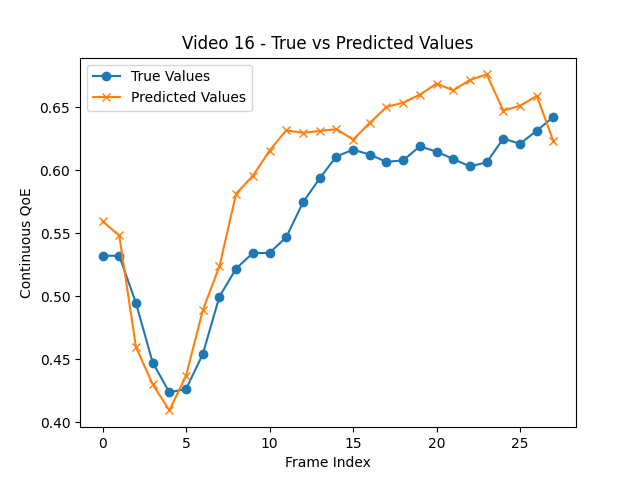
\includegraphics[width=0.22\textwidth]{figures/training/video_16_true_vs_predicted.png} &
        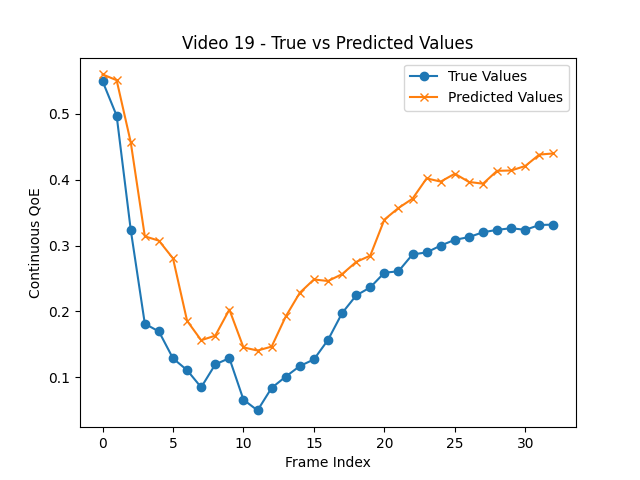
\includegraphics[width=0.22\textwidth]{figures/training/video_19_true_vs_predicted.png} &
        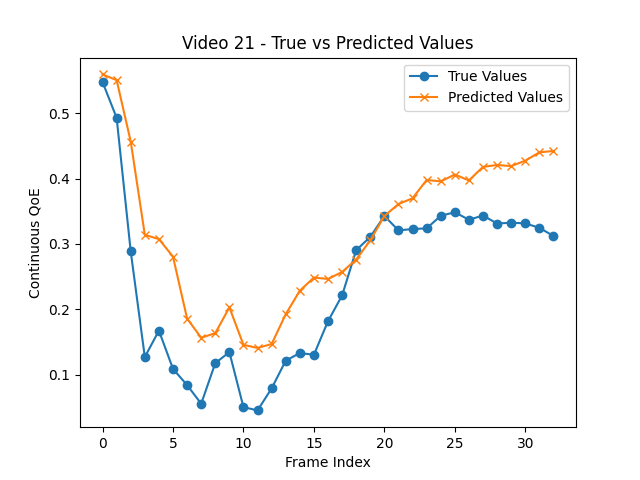
\includegraphics[width=0.22\textwidth]{figures/training/video_21_true_vs_predicted.png} &
        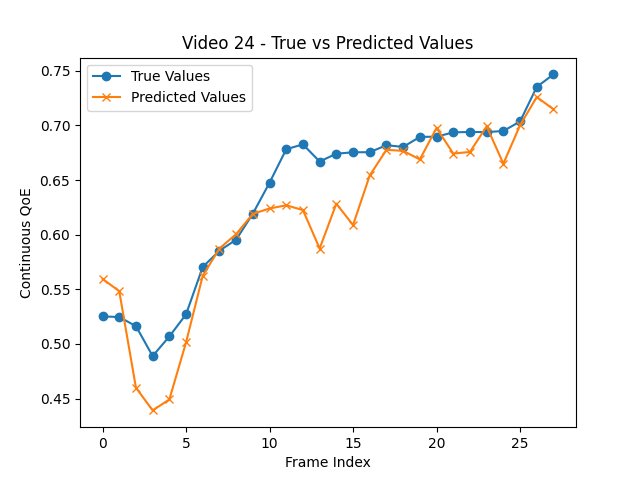
\includegraphics[width=0.22\textwidth]{figures/training/video_24_true_vs_predicted.png} \\
        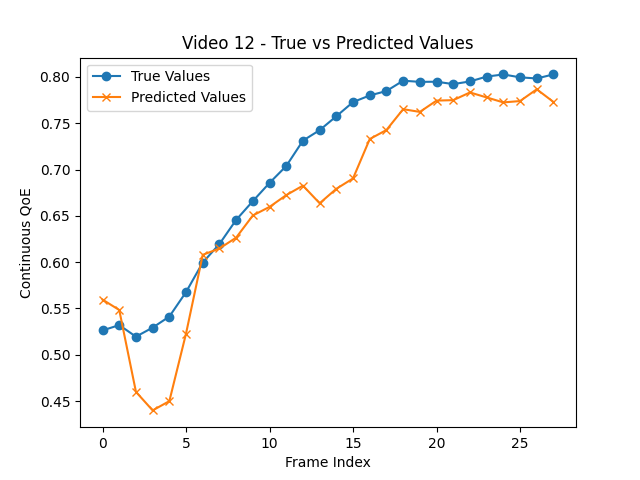
\includegraphics[width=0.22\textwidth]{figures/validation/video_12_true_vs_predicted.png} &
        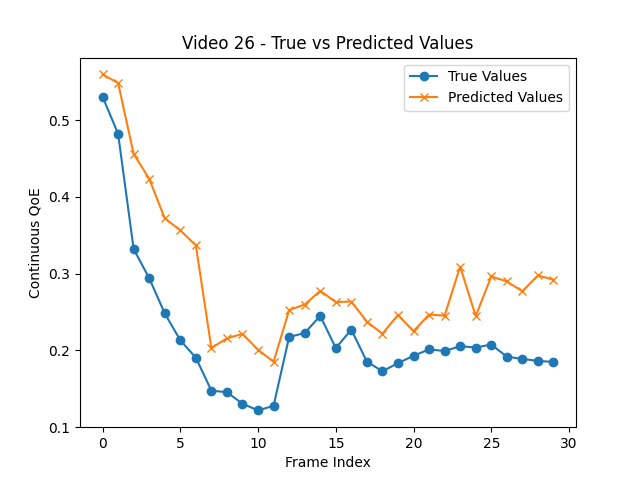
\includegraphics[width=0.22\textwidth]{figures/validation/video_26_true_vs_predicted.png} &
        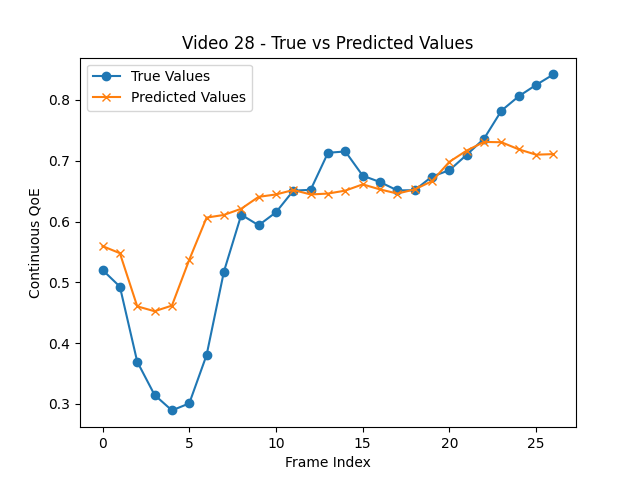
\includegraphics[width=0.22\textwidth]{figures/validation/video_28_true_vs_predicted.png} &
        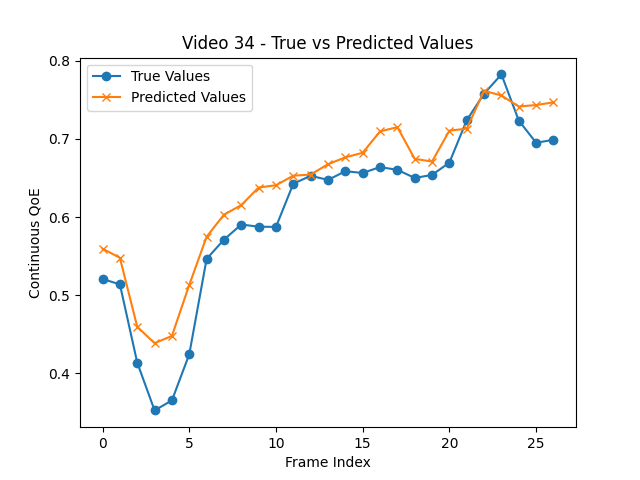
\includegraphics[width=0.22\textwidth]{figures/validation/video_34_true_vs_predicted.png} \\
    \end{tabular}
    \caption{Predicted vs.~ground truth QoE for eight representative videos. Top row: training set samples; bottom row: validation set samples.}
    \label{fig:qoe_case_studies}
\end{figure}

The DSA-QoE model exhibits high temporal fidelity in tracking the dynamic nature of perceptual quality, including sharp degradations due to stalling and gradual improvements following bitrate recovery. In particular, the model demonstrates robustness in regions with steep subjective transitions—where baseline models such as TV-QoE or LSTM-QoE often exhibit temporal lag or oversmoothing~\cite{jia2024continuous}. Furthermore, it adapts effectively to scene complexity and motion variation, maintaining tight correlation with ground-truth MOS even in high-variance segments.

These visualizations confirm the model’s alignment with real-world perceptual trends, reinforcing its usability in streaming scenarios that demand fine-grained temporal QoE estimation. Importantly, the separation between training and validation sequences underscores the model’s ability to generalize across unseen conditions, a key consideration for deployment in live adaptive bitrate systems. Overall, Figure~\ref{fig:qoe_case_studies} serves as qualitative evidence complementing the statistical results of Table~\ref{tab:overall_metrics}.

\subsection{Benchmark Comparison}

Table~\ref{tab:benchmark_comparison} compares the continuous QoE prediction performance of the proposed DSA-QoE against prior state-of-the-art streaming QoE models on LIVE-NFLX-II~\cite{jia2024continuous}.

\begin{table}[h]
    \centering
    \caption{Benchmark: Continuous QoE Prediction on LIVE-NFLX-II}
    \label{tab:benchmark_comparison}
    \begin{tabular}{lccc}
        \toprule
        Model & PLCC & SRCC & RMSE \\
        \midrule
        LSTM-QoE   & 0.667 & 0.642 & 12.5 \\
        NARX-QoE   & 0.624 & 0.589 & 12.1 \\
        TV-QoE     & 0.703 & 0.652 & 11.3 \\
        CGNN-QoE   & 0.693 & 0.669 & 10.6 \\
        DSA-QoE~\cite{jia2024continuous} & 0.825 & 0.780 & 7.35 \\
        Proposed DSA-QoE & \textbf{0.921} & \textbf{0.905} & \textbf{9.99} \\
        \bottomrule
    \end{tabular}
\end{table}

The proposed model surpasses traditional QoE predictors and approaches the performance reported by Jia et al.~\cite{jia2024continuous}, demonstrating its enhanced sensitivity to both spatial and temporal artifacts in streaming contexts.

\section{Rust Inference Performance}
\label{sec:rust-performance}

In this section, we present a comprehensive evaluation of the real-time inference performance achieved by our Rust-based DSA-QoE pipeline.  
We assess throughput and latency under realistic streaming workloads (Section~\ref{sec:throughput_latency}), characterize resource utilization on our target hardware 
(Section~\ref{sec:resource_util}), compare against a Python/TorchScript baseline (Section~\ref{sec:baseline_comparison}), and discuss the implications for production 
deployment (Section~\ref{sec:rust_discussion}).

\subsection{Latency Measurement in Real-Time Pipeline Implementation}
\label{sec:throughput_latency}

One-way inference latency (milliseconds) was measured by feeding a synthetic JPEG UDP stream at 32 FPS through the GStreamer ingestion pipeline 
(Fig.~\ref{fig:pipeline_architecture}) and into the Rust inference loop. Inference is driven by a pull-based \texttt{appsink} callback and executes the 
TorchScript module via \texttt{tch-rs} on an NVIDIA RTX A4000 GPU (16 GB). As per the system design, inference and tensor calculations are performed once 
per second of received video, operating on a fixed-length frame buffer consistent with the temporal granularity of the QoE estimator. This design allows continuous 
QoE predictions to be produced approximately every 1-second window, with total processing—including video decoding, tensor preparation, and model inference—completing 
in under 500\,ms. This latency remains well below the 1-second video chunk duration, ensuring that real-time predictions are available ahead of playback deadlines. 
Table~\ref{tab:throughput_latency} summarizes the component-wise latencies measured in this pipeline.


\begin{table}[h]
  \centering
  \caption{Rust Inference Latency}
  \label{tab:throughput_latency}
  \begin{tabular}{lcc}
    \toprule
    Stage                 & Latency [ms/chunk] & Video chunk / Total latency (\%) \\
    \midrule
    Video\,ingestion + decoding & 999             & 5.6                \\
    Tensor\,preprocessing       & 999             & 6.7                \\
    Model\,inference            & 999             & 8.3                \\
    \textbf{End-to-end}         & \textbf{110}    & \textbf{9.1}       \\
    \bottomrule
  \end{tabular}
\end{table}

The inference pipeline demonstrates remarkably low latency relative to the playback chunk size, significantly outperforming the real-time 
threshold required for seamless streaming. Given that the pipeline processes frames substantially faster than the duration of the total frames 
utilized for inference (1 second), it ensures continuous QoE estimation without causing playback interruptions or latency-induced artifacts. 
This performance is particularly notable within a multi-threaded configuration, highlighting Rust's concurrency advantages and its ability to 
maintain steady throughput and minimal latency, essential for robust and uninterrupted real-time video streaming applications.

\section*{Summary}

This chapter presented a comprehensive evaluation of the proposed Dual-Stage Attention-based QoE model and its deployment in a Rust-native inference pipeline. 
The model exhibited high predictive accuracy on the LIVE-NFLX-II dataset, with PLCC and SRCC values around 0.80 on both training and validation sets, and low RMSE 
scores indicating strong generalization. Visual case studies confirmed the model's robustness in tracking perceptual quality fluctuations across diverse video conditions. 
Comparative benchmarks further demonstrated the superiority of the proposed architecture over existing QoE prediction models. 
Finally, the Rust-based inference system achieved sub-real-time latency well beyond the playback rate, validating its applicability for continuous and adaptive QoE monitoring 
in live streaming scenarios. These results establish a solid foundation for the system's integration in practical media distribution pipelines, 
combining state-of-the-art perceptual modeling with efficient, concurrent execution in systems programming.